\documentclass[12pt, openany]{report}
\usepackage[utf8]{inputenc}
\usepackage[T1]{fontenc}
\usepackage{amsmath,amsfonts,amssymb}
\usepackage{amssymb}
\usepackage{multicol}
\usepackage[a4paper,left=2.5cm,right=2.5cm,top=2.5cm,bottom=2.5cm]{geometry}
\usepackage[english]{babel}
\usepackage{libertine}
\usepackage{graphicx}
\usepackage{wrapfig}
\usepackage{algorithm}
\usepackage{algpseudocode}
\usepackage{float}
\usepackage{enumitem}
\usepackage{pythonhighlight}
\usepackage[]{titletoc}
\usepackage{empheq}
\usepackage{titlesec}
\usepackage{mathpazo}
\usepackage{xfrac}
\usepackage{textcomp}
\usepackage{mathtools}
\usepackage{caption}
\usepackage{tabularray}
\usepackage{subcaption}
\usepackage[bottom]{footmisc}
\usepackage{pdfpages}
\usepackage{tabularx}
\usepackage{amsthm}
\usepackage[skins]{tcolorbox}
\titleformat{\chapter}[display]
  {\normalfont\bfseries}{}{0pt}{\Huge}
\usepackage{hyperref}
\newcommand{\hsp}{\hspace{20pt}}
\newcommand{\HRule}{\rule{\linewidth}{0.5mm}}
\newcommand{\R}{\mathbb{R}}
\newcommand{\C}{\mathbb{C}}
\theoremstyle{definition}
\newtheorem{thm}{Theorem}[chapter]
\newtheorem{definition}[thm]{Definition}
\newtheorem{lem}[thm]{Lemma}

\hbadness=100000
\begin{document}
\begin{titlepage}
    \begin{sffamily}
    \begin{center}
        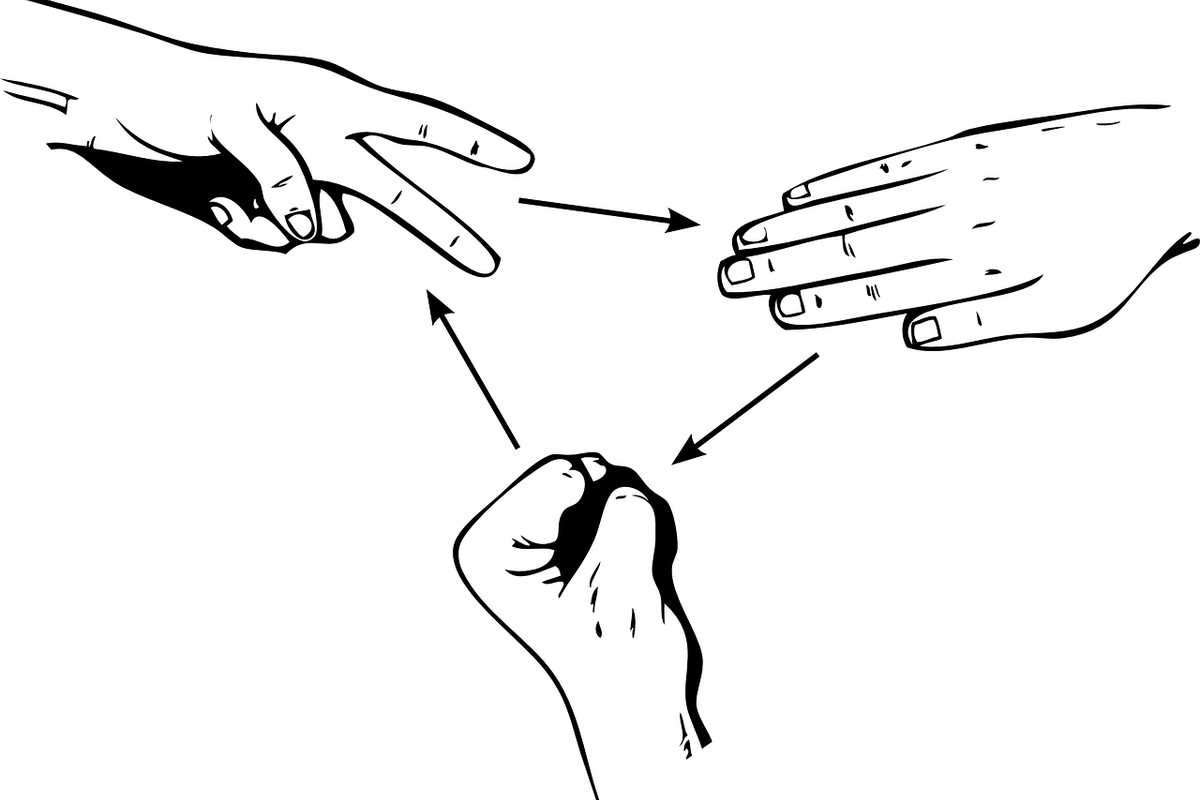
\includegraphics[scale=0.25]{img/page_de_garde.png} \\[1cm]
        \HRule \\[0.4cm]
        { \huge \bfseries LINMA2345 Game Theory \\[0.4cm] }
    
        \HRule \\[1.5cm]
        \textsc{\LARGE Simon Desmidt}\\[1cm]
        \vfill
        \vspace{2cm}
        {\large Academic year 2024-2025 - Q2}
        \vspace{0.4cm}
         
        
\includegraphics[width=0.15\textwidth]{img/epl.png}
        
        UCLouvain\\
    
    \end{center}
    \end{sffamily}
\end{titlepage}

\setcounter{tocdepth}{1}
\tableofcontents
\chapter{Basic models}
In a model, we need to define the actions, the knowledge, the randomness and the outcomes. \\
A private information is any knowledge on the state of the world that is not a common knowledge. An information $X$ is said to be common knowledge if the statement (everybody knows that$)^{K}$ everybody knows $X$ holds for any integer $K$
\section{Extensive form games}
The extensive form is a tree. The nodes trigger something: they can be triggered by a player of by chance. The edges are the actual events of the game, from a player or from chance. The leaves are the payoffs, containing one item per player. 
\begin{figure}[H]
  \centering 
  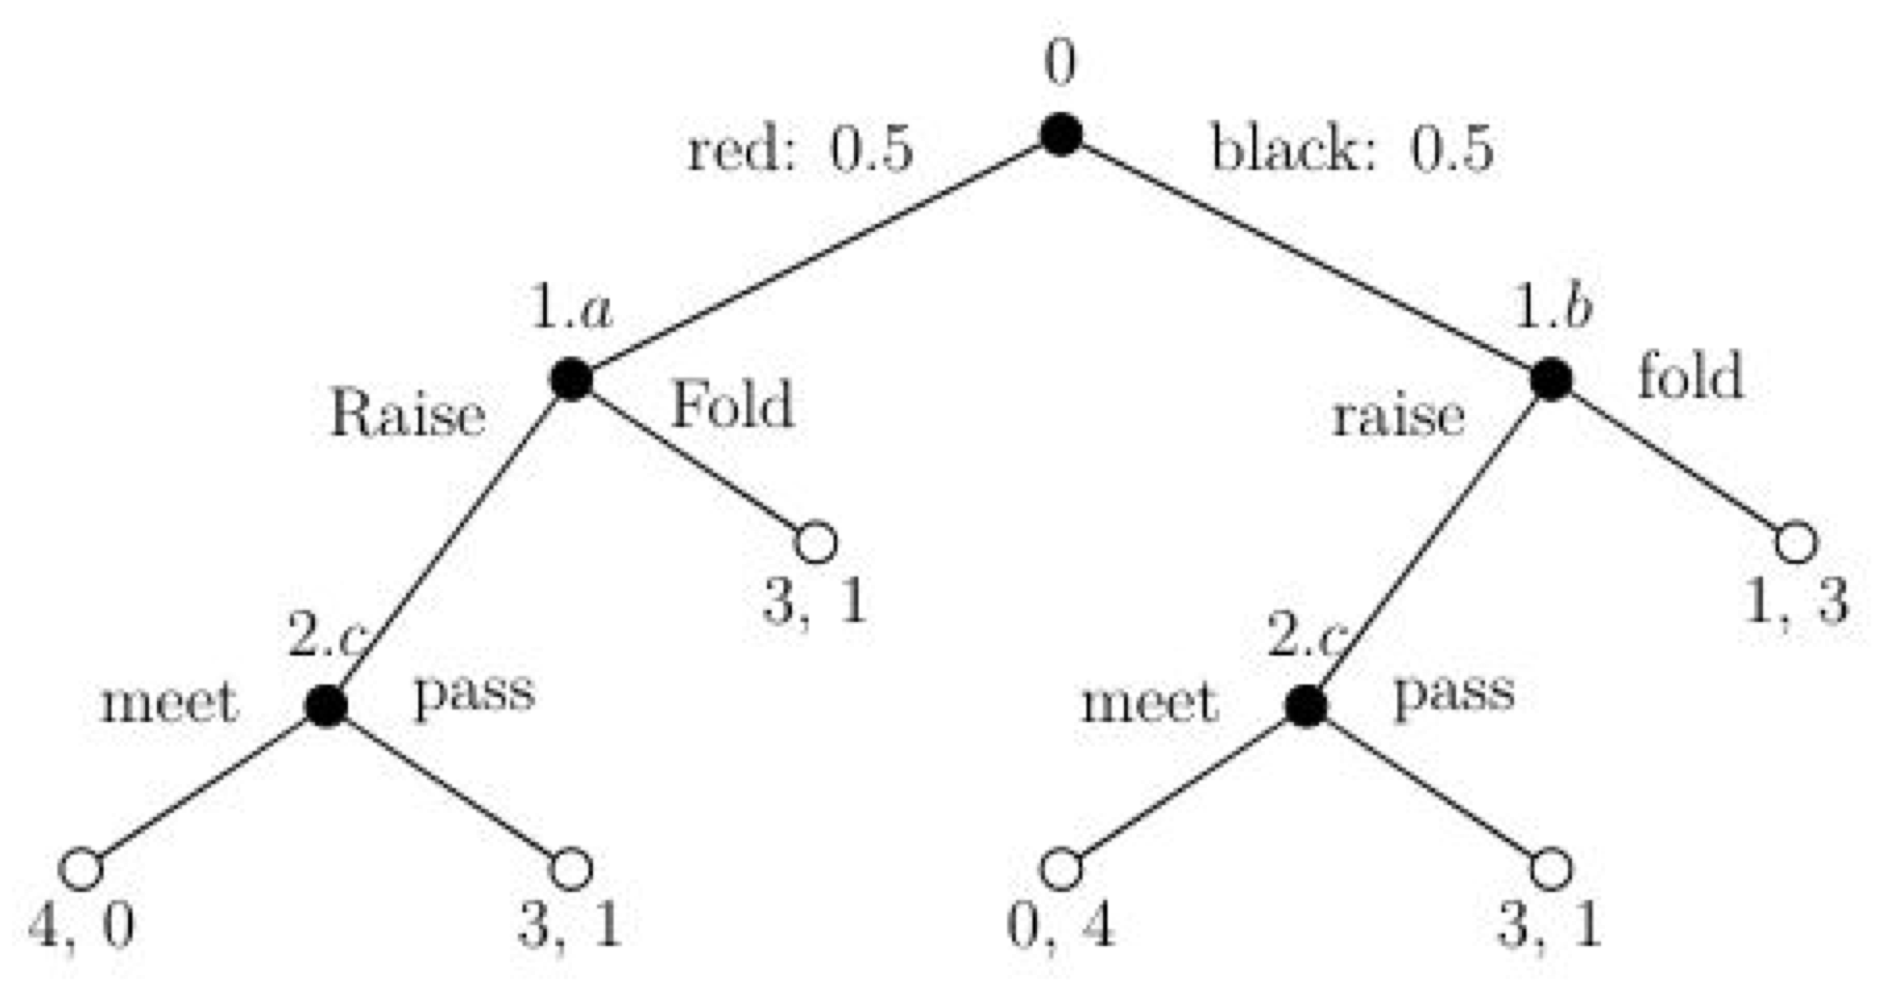
\includegraphics[scale=.15]{img/extensive.png}
\end{figure}
The extensive form contains the following elements:
\begin{itemize}
	\item $N$: the set of players (e.g. by name);
	\item $S$: the set of information states, i.e. the information to which each player has access;
	\item $D$: the set of moves for a player that is at a certain information states (meet or pass, raise or stop, etc.);
	\item $V$: the set of nodes (e.g. numbered);
	\item $V_0$: the set of chance nodes;
	\item $Y$: the set of action nodes, i.e. where someone does something;
	\item $X$: the set of leaves;
	\item $t$: the transitions, i.e. the outgoing edges from a node;
	\item $p$: the probability distribution for the random transitions;
	\item $w$: the payoffs for each player at each leaf.
\end{itemize}
\subsection{Concepts}
\begin{itemize}
	\item Perfect recall: Players remember their past states and moves;
	\item Perfect information: Every player knows where they are in the game;
	\item Pure strategy: A function associates a move to each information state, i.e. if something happens, the strategy says what to do next;
	\item Payoff of a strategy: It is the expected final value, i.e. the probability of an result times its payoff;
	\item Randomized strategy: We assign, at each information state, a probability distribution on the moves.
\end{itemize}
\section{Strategic form games}
A strategic game is a tuple $\Gamma=(N,C,u)$ where $N$ is the set of players, $C$ the set of pure strategies for all players, and $u$ the payoff function. Using a randomized strategy, we have the following expected payoff formula, with the probability distribution $\sigma_i$:
\begin{equation}
	E_\sigma (u_i(c)) = \sum_{c\in C}\sigma(x)u_i(x) = \sum_{c_i\in C_i} \sigma_i(c_i)\sum_{c_{-i}\in C_{-i}}\sigma_{-i}(c_{-i})u_i(c_i,c_{-i})
\end{equation}
where $-i$ denotes the set of all players except $i$, and $\sigma_{-i}(c_{-i}) =\prod_{j\neq i}\sigma_j(c_j)$.\\
Consider a player $i\in N$. If the players $-i$ play following the strategy profile $\sigma_{-i}$, then the set of best response strategies for player $i$ is given by 
\begin{equation}
	\arg\max_{c_i\in C_i} \sum_{c_{-i}\in C_{-i}}\sigma_{-i}(c_{-i})u_i(c_i,c_{-i})
\end{equation}
\subsection{Strong domination}
A strategy is strongly dominated if it cannot be a best response. 
\begin{figure}[H]
	\centering 
	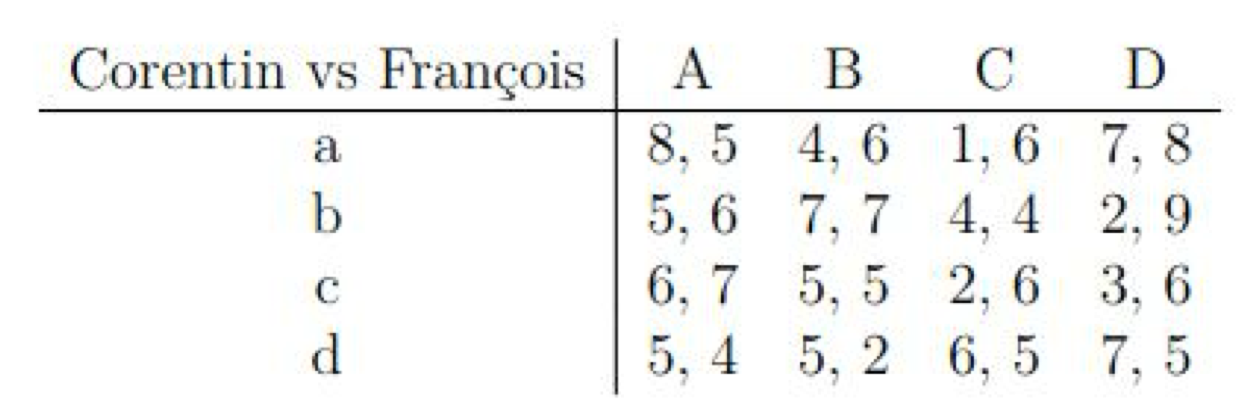
\includegraphics[scale=.15]{img/strong_dom.png}
\end{figure}
It means that, for a given column, there exists another one where all the second numbers are strictly bigger than in the considered one. This works too for the rows, using the first numbers. In that case, the column or row can be completely removed, as the player never has an interest in using that strategy. In the example above, column B is strongly dominated by column D.
\begin{itemize}
	\item [$\rightarrow$] Note: once a column or row has been removed, we can continue to iterate on the smaller table until no row or column can be removed again. The convergence to a certain table is guaranteed, whatever the order of removal.
\end{itemize}
\subsection{Weak domination}
Weak domination changes the strictly bigger into a bigger or equal. In that case, it is not always a good move to remove the strategy, particularly if the game includes randomness. 
\begin{itemize}
	\item [$\rightarrow$] Note: Removing the weakly dominated strategies does not conserve convergence. 
\end{itemize}
\section{Equivalent models}
Two games are fully equivalent if 
\begin{equation}
	\forall i \in N, \ \exists A_i>0, B_i\ : \ \hat u_i(c) = A_iu_i(c)+B_i \qquad \forall c\in C
\end{equation}
This means that the scale of the payoffs changes nothing. 
\subsection{Best-reponse equivalence}
Two games are best-response equivalent iff they have the best response sets, i.e.
\begin{equation}
	c_i'\in \arg\max_{c_i\in C_i} \sum_{c_{-i}\in C_{-i}} \sigma_{-i}(c_{-i})u_i(c_i,c_{-i}) \iff c_i'\in \arg\max_{c_i\in C_i} \sum_{c_{-i}\in C_{-i}} \sigma_{-i}(c_{-i})\hat u_i(c_i,c_{-i})
\end{equation}
\section{Bayesian game}
In a Bayesian game, we add the set of player types $T$ and the belief functions. What was before a set of players is now a set of agents, each of which is a player in a certain state depending on the randomness of some piece of information.
\section{Nash Equilibrium}
\subsection{Definitions}
\begin{itemize}
	\item Given a game in extensive form $\Gamma_e$, a pure strategy for a player $i\in N$ is an element $c\in C_i = \times_{s\in S_i}D_s$, acting as a function that associates to each information state of the player a move to be played at that state. A pure strategy is such that, for any move of the opponent(s) and at any time in the game, it prescribes a move to be played.
	\item A randomized strategy $(\sigma_1,\dots, \sigma_N)$ consists in choosing one of the pure strategies with a certain probability. For example, in rock paper scissors, a strategy is to do one of the three possibilities with probability 1/3 for each.\\
	They verify the following conditions:
	\begin{equation}
		\begin{aligned}
			&\sum_{c_i\in D_i}\sigma_i(c_i)=1\\
			\forall d_i\in D_i\ :\qquad &\sigma_i(d_i)\ge 0\\
			\forall e_i\in C_i\setminus D_i\ : \qquad &\sigma_i(e_i)=0\\
		\end{aligned}
	\end{equation}
	\item A Nash equilibrium is such that no player alone has an interest to deviate from his current situation. For example, in the prisoner's dilemma, the Nash equilibrium is that both players defect, because none of them can decide to cooperate and have a higher payoff.\\
	In a Nash equilibrium, all strategies are best responses to $\sigma_{-i}$, and thus they payoffs are equal:
	\begin{equation}
		\begin{aligned}
			\forall d_i\in D_i\ : \qquad &\sum_{c_{-i}\in D_{-i}} \left(\prod_{j\in N-i}\sigma_j(c_j)\right) u_i(c_{-i},d_i)=w_i\\
			\forall e_i\in C_i\setminus D_i\ : \qquad &\sum_{c_{-i}\in D_{-i}} \left(\prod_{j\in N-i}\sigma_j(c_j)\right) u_i(c_{-i},e_i)\le w_i
		\end{aligned}
	\end{equation}
	\item [$\to$] Note: the product in those equations corresponds to the probabilities of the other players strategies, and the $u_i$ next to it correspond to the rewards considering each player's strategy. The first equation means that all selected strategies have the same payoff, and the second one means that all strategies are the best response. 
	\item The support of a game consists in the set of all possible combinations of strategies for all players. It can contain pure strategies as well as randomized strategies. 
	\item A zero-sum game is such that the sum of payoffs is equal to zero in all situations, i.e. some players win what the other lose.
\end{itemize}
\section{Properties}
\begin{itemize}
	\item There always exists at least one Nash equilibrium.
	\item If there exists more than one Nash equilibrium in pure strategies, then there exists an infinity of them in randomized strategies, as any linear combination of the Nash equilibria is also a Nash equilibrium.
	\item Given a two-person zero-sum game $\Gamma({1,2},(C_1,C_2), (u_1,-u_1))$, the strategy profile $\sigma=(\sigma_1,\sigma_2)$ is a Nash equilibrium iff 
	\begin{equation}
		\sigma_1\in \arg\max_{\tau_1\in \Delta (C_1)}\min_{\tau_2\in \Delta (C_2)}u_1(\tau_1,\tau_2)
	\end{equation}
	and 
	\begin{equation}
		\sigma_2\in \arg\min_{\tau_2\in \Delta (C_2)}\max_{\tau_1\in \Delta (C_1)}u_1(\tau_1,\tau_2)
	\end{equation}
	If $(\sigma_1,\sigma_2)$ is a Nash equilibrium, then 
	\begin{equation}
		u_1(\sigma_1,\sigma_2)= \max_{\tau_1\in \Delta (C_1)}\min_{\tau_2\in \Delta (C_2)}u_1(\tau_1,\tau_2)=\min_{\tau_2\in \Delta (C_2)}\max_{\tau_1\in \Delta (C_1)}u_1(\tau_1,\tau_2) 
	\end{equation}
	\item In a game containing $N$ players and $M$ moves, the total number of pairs of strategies is $(2^M-1)^N$. 
\end{itemize}
\section{How to find them}
\begin{itemize}
	\item Remove all strongly dominated strategies;
	\item Check if some of the remaining strategies will never be played, whatever the opponents choose. 
\end{itemize}
\section{Drawbacks}
\begin{itemize}
	\item There is no way to choose between the several equilibria, when there are more than one.
	\item No communication between agents can lead to a non optimal solution (see for example the prisoner's dilemma).
	\item The table form when looking for equilibria does not display all the information of the game.
	\item Finding the equilibria can be computationnally intensive.
\end{itemize}
\end{document}